% This template has been tested with LLNCS DOCUMENT CLASS -- version 2.20 (24-JUN-2015)

%"runningheads" enables:
%  - page number on page 2 onwards
%  - title/authors on even/odd pages
%This is good for other readers to enable proper archiving among other papers and pointing to
%content. Even if the title page states the title, when printed and stored in a folder, when
%blindly opening the folder, one could hit not the title page, but an arbitrary page. Therefore,
%it is good to have title printed on the pages, too.
\documentclass[runningheads,a4paper]{llncs}[2015/06/24]

%cmap has to be loaded before any font package (such as cfr-lm)
\usepackage{cmap}
\usepackage[T1]{fontenc}

%https://tex.stackexchange.com/questions/57743/how-to-write-%c3%a4-and-other-umlauts-and-accented-letters-in-bibliography#57745
%for german umlauts
\usepackage[utf8]{inputenc}

\usepackage{graphicx}

%Even though `american`, `english` and `USenglish` are synonyms for babel package (according to https://tex.stackexchange.com/questions/12775/babel-english-american-usenglish), the llncs document class is prepared to avoid the overriding of certain names (such as "Abstract." -> "Abstract" or "Fig." -> "Figure") when using `english`, but not when using the other 2.
%english has to go last to set it as default language
\usepackage[ngerman,english]{babel}
%Hint by http://tex.stackexchange.com/a/321066/9075 -> enable "= as dashes
\addto\extrasenglish{\languageshorthands{ngerman}\useshorthands{"}}

%better font, similar to the default springer font
%cfr-lm is preferred over lmodern. Reasoning at http://tex.stackexchange.com/a/247543/9075
\usepackage[%
rm={oldstyle=false,proportional=true},%
sf={oldstyle=false,proportional=true},%
tt={oldstyle=false,proportional=true,variable=true},%
qt=false%
]{cfr-lm}
%
%if more space is needed, exchange cfr-lm by mathptmx
%\usepackage{mathptmx}

%for demonstration purposes only
\usepackage[math]{blindtext}

%Sorts the citations in the brackets
%It also allows \cite{refa, refb}. Otherwise, the document does not compile.
%  Error message: "White space in argument"
\usepackage{cite}


%% If you need packages for other papers,
%% START COPYING HERE
%% COPY ALSO cmap and fontenc from lines 10 to 12

%extended enumerate, such as \begin{compactenum}
\usepackage{paralist}

%put figures inside a text
%\usepackage{picins}
%use
%\piccaptioninside
%\piccaption{...}
%\parpic[r]{\includegraphics ...}
%Text...

%for easy quotations: \enquote{text}
\usepackage{csquotes}

%enable margin kerning
\usepackage{microtype}

%tweak \url{...}
\usepackage{url}
%\urlstyle{same}
%improve wrapping of URLs - hint by http://tex.stackexchange.com/a/10419/9075
\makeatletter
\g@addto@macro{\UrlBreaks}{\UrlOrds}
\makeatother
%nicer // - solution by http://tex.stackexchange.com/a/98470/9075
%DO NOT ACTIVATE -> prevents line breaks
%\makeatletter
%\def\Url@twoslashes{\mathchar`\/\@ifnextchar/{\kern-.2em}{}}
%\g@addto@macro\UrlSpecials{\do\/{\Url@twoslashes}}
%\makeatother

%diagonal lines in a table - http://tex.stackexchange.com/questions/17745/diagonal-lines-in-table-cell
%slashbox is not available in texlive (due to licensing) and also gives bad results. This, we use diagbox
%\usepackage{diagbox}

%required for pdfcomment later
\usepackage{xcolor}


%enable nice comments
%this also loads hyperref
\usepackage{pdfcomment}
%enable hyperref without colors and without bookmarks
\hypersetup{hidelinks,
   colorlinks=true,
   allcolors=black,
   pdfstartview=Fit,
   breaklinks=true}
%enables correct jumping to figures when referencing
\usepackage[all]{hypcap}

\newcommand{\commentontext}[2]{\colorbox{yellow!60}{#1}\pdfcomment[color={0.234 0.867 0.211},hoffset=-6pt,voffset=10pt,opacity=0.5]{#2}}
\newcommand{\commentatside}[1]{\pdfcomment[color={0.045 0.278 0.643},icon=Note]{#1}}

%compatibality with packages todo, easy-todo, todonotes
\newcommand{\todo}[1]{\commentatside{#1}}
%compatiblity with package fixmetodonotes
\newcommand{\TODO}[1]{\commentatside{#1}}

%enable \cref{...} and \Cref{...} instead of \ref: Type of reference included in the link
\usepackage[capitalise,nameinlink]{cleveref}
%Nice formats for \cref
\crefname{section}{Sect.}{Sect.}
\Crefname{section}{Section}{Sections}

\usepackage{xspace}
%\newcommand{\eg}{e.\,g.\xspace}
%\newcommand{\ie}{i.\,e.\xspace}
\newcommand{\eg}{e.\,g.,\ }
\newcommand{\ie}{i.\,e.,\ }

%introduce \powerset - hint by http://matheplanet.com/matheplanet/nuke/html/viewtopic.php?topic=136492&post_id=997377
\DeclareFontFamily{U}{MnSymbolC}{}
\DeclareSymbolFont{MnSyC}{U}{MnSymbolC}{m}{n}
\DeclareFontShape{U}{MnSymbolC}{m}{n}{
    <-6>  MnSymbolC5
   <6-7>  MnSymbolC6
   <7-8>  MnSymbolC7
   <8-9>  MnSymbolC8
   <9-10> MnSymbolC9
  <10-12> MnSymbolC10
  <12->   MnSymbolC12%
}{}
\DeclareMathSymbol{\powerset}{\mathord}{MnSyC}{180}

% correct bad hyphenation here
\hyphenation{op-tical net-works semi-conduc-tor}

%% END COPYING HERE

\usepackage{subfigure}


\begin{document}

\title{Bilderkennung mit Convolutional Neural Networks}
%If Title is too long, use \titlerunning
%\titlerunning{Short Title}

%Single insitute
\author{Ivo Tremel \and Lennard Nöhren}
%If there are too many authors, use \authorrunning
%\authorrunning{First Author et al.}
\institute{Computational Health Informatics}

%Multiple insitutes
%Currently disabled
%
\iffalse
%Multiple institutes are typeset as follows:
\author{Firstname Lastname\inst{1} \and Firstname Lastname\inst{2} }
%If there are too many authors, use \authorrunning
%\authorrunning{First Author et al.}

\institute{
Insitute 1\\
\email{...}\and
Insitute 2\\
\email{...}
}
\fi
			
\maketitle

\begin{abstract}
Wir haben ein aufs Wesentliches reduziertes Faltungsnetz zur Klassifizierung von je 100  verschiedenen, handschriftlichen Buchstaben
in zehn verschiedene Kategorien trainiert. Dabei wurde eine Genauigkeit von 85\% erreicht. Das convolutional neural network (CNN) besteht aus einer Faltungsebene, die von einer Max-Pooling Ebene und einer Fully-Connected Ebene gefolgt wird. Zudem wurde die Erweiterung der Inception-Layers verwendet.
\end{abstract}

\begin{keywords}
keyword1, keyword2
\end{keywords}

%%%%%%%%%%%%%%%%%%%%%%%%%%%%%%%%%%%%%%%%%%%%%%%%%%%%%%%%%%%%%%%%%%%%%%%%%%%%%%%
\section{Introduction}\label{sec:intro}
%%%%%%%%%%%%%%%%%%%%%%%%%%%%%%%%%%%%%%%%%%%%%%%%%%%%%%%%%%%%%%%%%%%%%%%%%%%%%%%
%Convolutional Neural Networks kommen nahe an menschliche Leistungen heran und der Ansatz der Faltungsnetze bewahrt die entscheidende Lokalität der Bildinformationen. Allerdings
Das Erkennen von handschriftlichen Texten in Echtzeit ist eine Funktion, die in vielen Bereichen genutzt werden könnte. Allerdings muss man dafür eine präzise Bildanalyse durchführen, was im Allgemeinen einen hohen Rechenaufwand mit sich bringt. In den letzten Jahren hat der sehr schnelle Fortschritt in dem Bereich Machine Learning und insbesondere Neuronale Netze allerdings eine gute Lösung für diese Problematik hervorgebracht. Convolutional Neural Networks (kurz: CNN) haben großartige Ergebnisse bei allen möglichen Arten der Bildanalyse gezeigt und sind auch ausgezeichnet zum Erkennen von Buchstaben geeignet. Es werden auch immer wieder neue Verbesserungen für CNN's entwickelt, welche die Präzision der Klassifizierung und die Laufzeit stetig verbessern. Eine dieser Erweiterungen sind die so genannten Inception Module, welche im Jahr 2014 das erste mal in GoogLeNet verwendet wurden \cite{inception_paper}.\\
Im folgenden wird ein klassisches CNN und ein CNN mit einem Inception Modul für eine Zeichenerkennung genutzt und die Performance der Beiden Netze wird verglichen.\\
Als zusätzliche Erschwerung enthält das Datenset auch die deutschen Umlaute \"{A} \"{O} und \"{U}, welche nur besonders schwer von den Buchstaben A O und U zu unterscheiden sind.
\section{Datensatz}\label{sec:dataset}
Der genutzte Datensatz besteht aus 1000 handschriftlichen Buchstaben, die in 10 Klassen klassifiziert werden können. Die Klassen bestehen aus den Buchstaben A,M,O,T,U und Ä,Ö,Ü,Y,V.Allerdings mussten wir feststellen, dass einige Labels falsch sind. Bei dem Bild \glqq image\_Ä\_up\_106\_point\_24.png \grqq ist z.B. kein Ä, sondern ein A zu erkennen.
\begin{figure}
	\caption{Falsch gelabeltes Ä}
	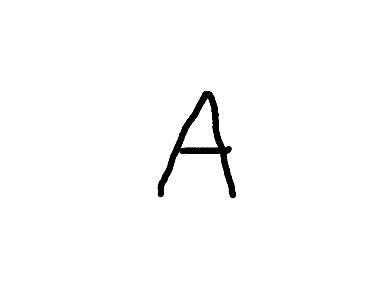
\includegraphics[width=0.5\textwidth]{hand_images/image_Ae_up_106_point_24.png}
	\label{fig:main_graph}
\end{figure}

\section{Materials and Methods}\label{sec:material}

\subsection{Klassische Convolutional Neural Networks}
CNNs sind für die Verarbeitung von Daten, die aus mehreren Arrays bestehen, konstruiert. Dies ist zum Beispiel bei einem Farbbild, welches aus drei 2D Arrays besteht, der Fall. In den Arrays des Farbbildes stehen dabei die Pixel Intensitäten der Farbkanäle. Es gibt vier zentrale Ideen bei CNNs, die die Eigenschaften von natürlichen Signalen ausnutzen. Dazu gehören die lokalen Verbindungen, die getielten Gewichte, das Pooling und die Nutzung von vielen Layers \cite{lecun_nature}. In Bilddaten korrelieren lokale Gruppen von Daten oft sehr stark und bilden damit unterscheidbare lokale Motive, die leicht erkennbar sind. Die Rolle der Convolution Layers ist die Entdeckung von lokalen Features des vorherigen Layers. Die Pooling Layers haben die Aufgabe semantisch gleiche Features in eins zusammenzuführen.

Bei der Nutzung von tiefen neuronalen Netzen wird die Eigenschaft ausgenutzt, dass viele natürliche Signale aus zusammengesetzten Hierarchien bestehen. Bei Bildern werden aus lokalen Kombinationen von Kanten Motive geformt. Diese können wiederum zu Objekten zusammengeführt werden. Die Convolution und Pooling Layers in CNNs sind direkt durch die Abläufe von einfachen und komplexen Zellen der visuellen Neurowissenschaft inspiriert. Die gesamte Architektur hat Paralellitäten zu der Hierarchie des visuellen Cortex. 

\subsubsection*{Convolutional Layers:}
Die Neuronen im Convolutional Layer führen eine diskrete Faltung auf dem Eingabebild durch. Dafür verwenden sie eine kleine Matrix, zum Beispiel mit der Größe 5x5, mit der sie über das Bild laufen und jeweils durch das innere Produkt der Matrix die Werte berechnen. Diese Matrix wird Fitlerkernel genannt. Danach wird wie bei normalen Neuronen mithilfe einer Aktivierungsfunktion der Output des Neurons bestimmt. Der Vorteil dieser Methode ist, das durch den Filterkernel nicht nur einzelne Punkte eines Bildes betrachtet werden, sondern auch die lokale Umgebung von jedem Punkt. Dadurch können größere Features, die aus mehreren Punkten bestehen besser erkannt werden.

\subsubsection*{Pooling Layers:}
In CNNs fassen Pooling-Layers den Output von den vorhergehenden Neuronen entsprechend der gewählten Kernelgröße zusammen. Dabei wird bei einem 2x2 Kernel der größte Output durchgeschaltet und die anderen drei Ausgänge verworfen. Damit wird eine Reduktion der Datenmenge erreicht, die eine insgesamt schnellere Berechnung ermöglicht.

\subsubsection*{Aufbau:}
\begin{figure}
	\caption{Main Graph of Classic CNN}
	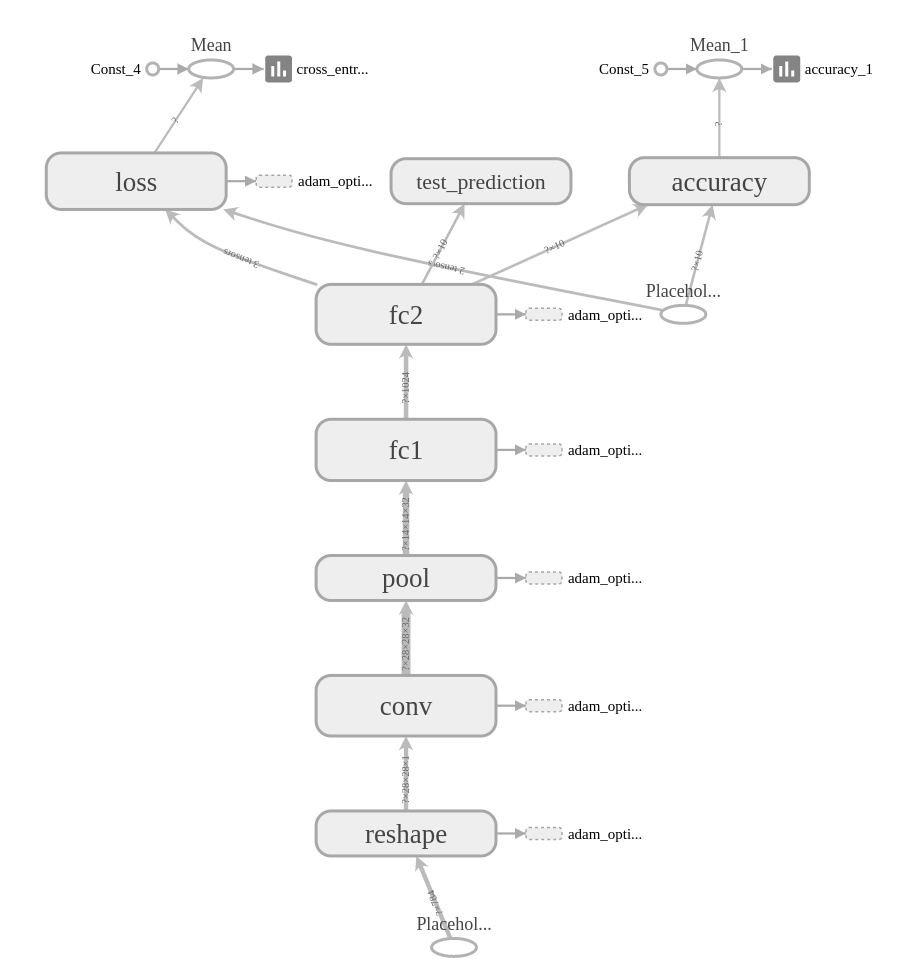
\includegraphics[width=\textwidth]{images/main_graph_conv.png}
	\label{fig:main_graph}
\end{figure}
\Cref{fig:main_graph} zeigt den Aufbau des CNNs. Vor dem ersten Convolutional Layer wird das Eingabebild zu einem 28x28x1 Bild transformiert. Die erste und zweite Dimension stehen dabei für die Bildhöhe und Bildbreite. Die dritte Dimension bezeichnet die Anzahl von Farbkanälen. Da es sich um ein Graustufenbild handelt und nicht RGB wird der Wert 1 angenommen. 
Bei der convolution werden mit einer Kernelgröße von 5x5 32 features erzeugt. Danach wird ein max-pooling mit einer Kernelgröße von 2x2 und einer Schrittweite von 2 durchgeführt. Dadurch wird die Größe des Bildes auf 14x14 reduziert. Anschließend werden die features in ein fully-connected Layer weitergeleitet. Dort werden die Daten in 1024 Nodes verarbeitet und danach an das Output layer, welches ein fully-connected Layer mit 10 Outputs ist, übergeben. Jeder Output steht dabei für einen Buchstaben.

\subsection{CNN mit Inception Layer}
\subsubsection*{Inception Layers:}
\begin{figure}
	\caption{Aufbau eines Inception Layers}
	\subfigure[Naiver Aufbau]{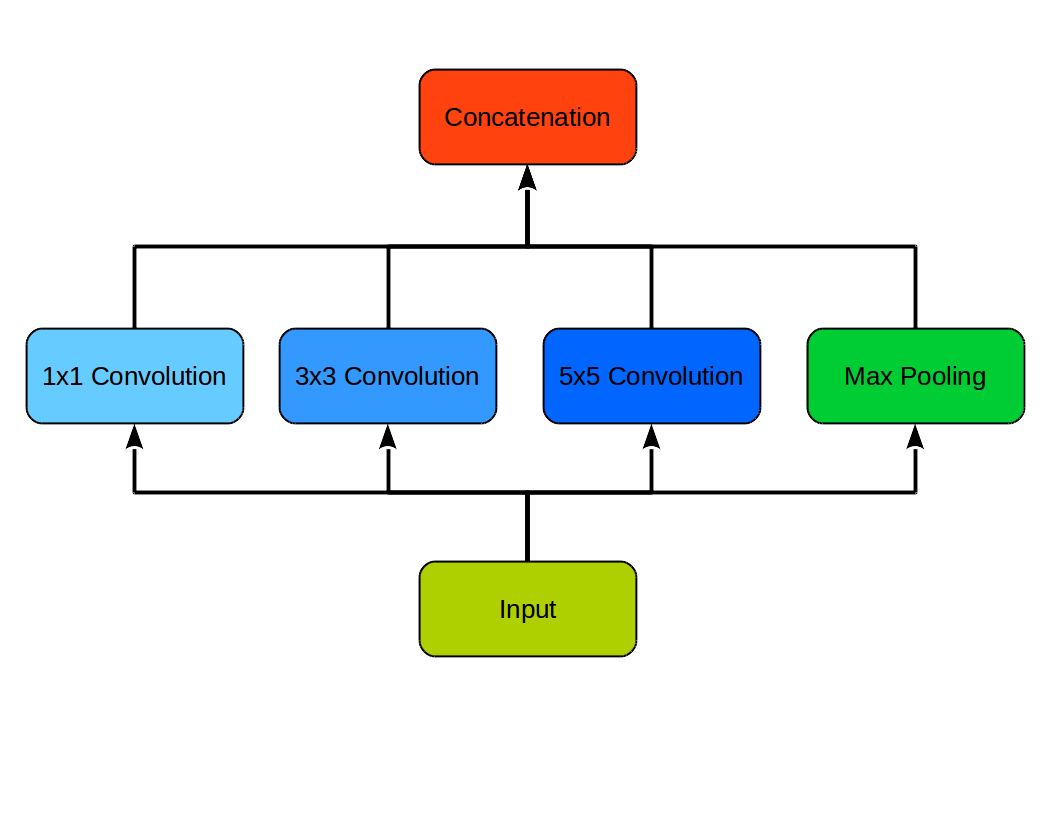
\includegraphics[width=0.49\textwidth]{images/inception_naive_graph.png}}
	\subfigure[Verbesserter Aufbau]{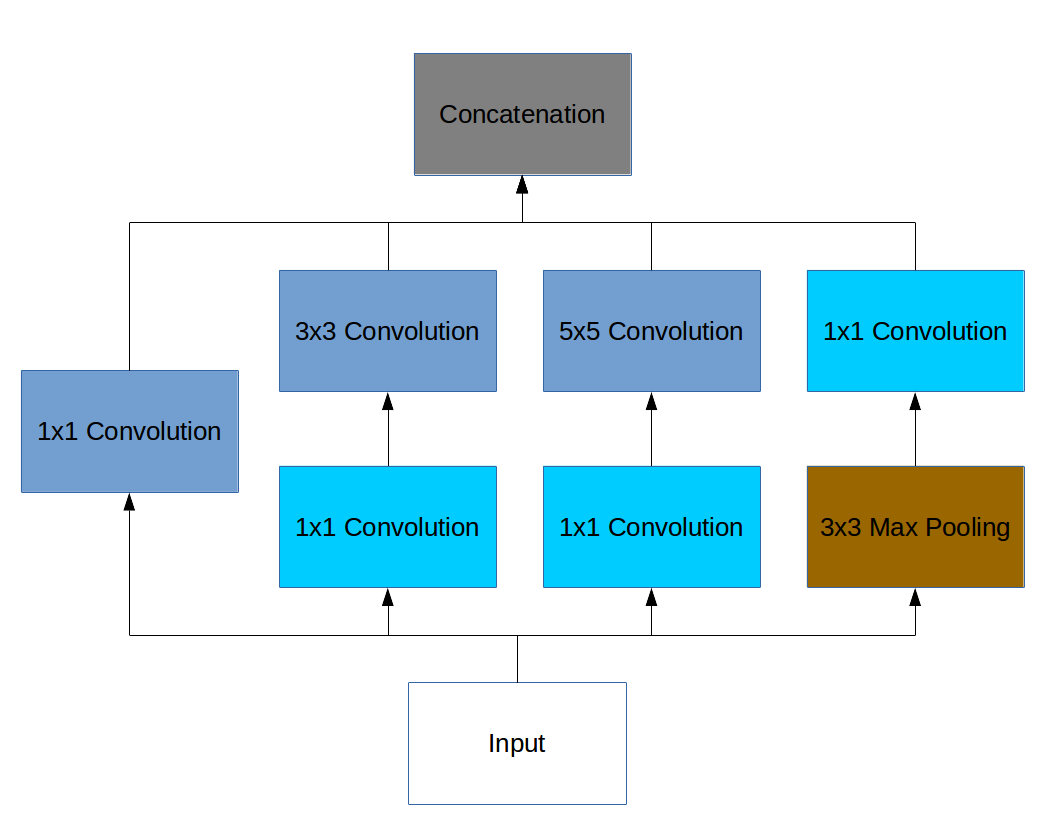
\includegraphics[width=0.49\textwidth]{images/inception_pro_graph.png}}
	\label{fig:inception_graph}
\end{figure}
In einem normalen Convolutional Layer muss festgelegt werden welche Größe der Filterkernel haben soll. Verschieden Größen bringen dabei immer Vor- und Nachteile mit sich. Deshalb ist die Idee von Inception Layers diese Wahl flexibler zu machen und dem Netz zu überlassen. Um das zu ermöglichen enthält ein Inception Layer Convolution Module mit verschiedenen Kernelgrößen und auch pooling Module, die Konkateniert werden.
In \Cref{fig:inception_graph} sieht man den Aufbau eines Inception Layers. Links ist zunächst der Naive Aufbau, wobei alle Module direkt auf den Input angewendet und dann Konkateniert werden. Das Problem bei diesem Ansatz ist allerdings, das dieses Layer einen extrem hohen Rechenaufwand hätte. Um diesen ein wenig zu verringern führt man üblicherweise vor den großen Convolutions jeweils auch eine 1x1 Convolution durch. Durch die 1x1 Convolution reduziert man die Dimension des Inputs für die großen Module, was zu einer deutlich besseren Laufzeit führt. Dadurch erhält man den Aufbau, den man in dem rechtem Diagramm sieht.

\subsubsection*{Aufbau:}
\begin{figure}
	\caption{Main Graph of Inception CNN}
	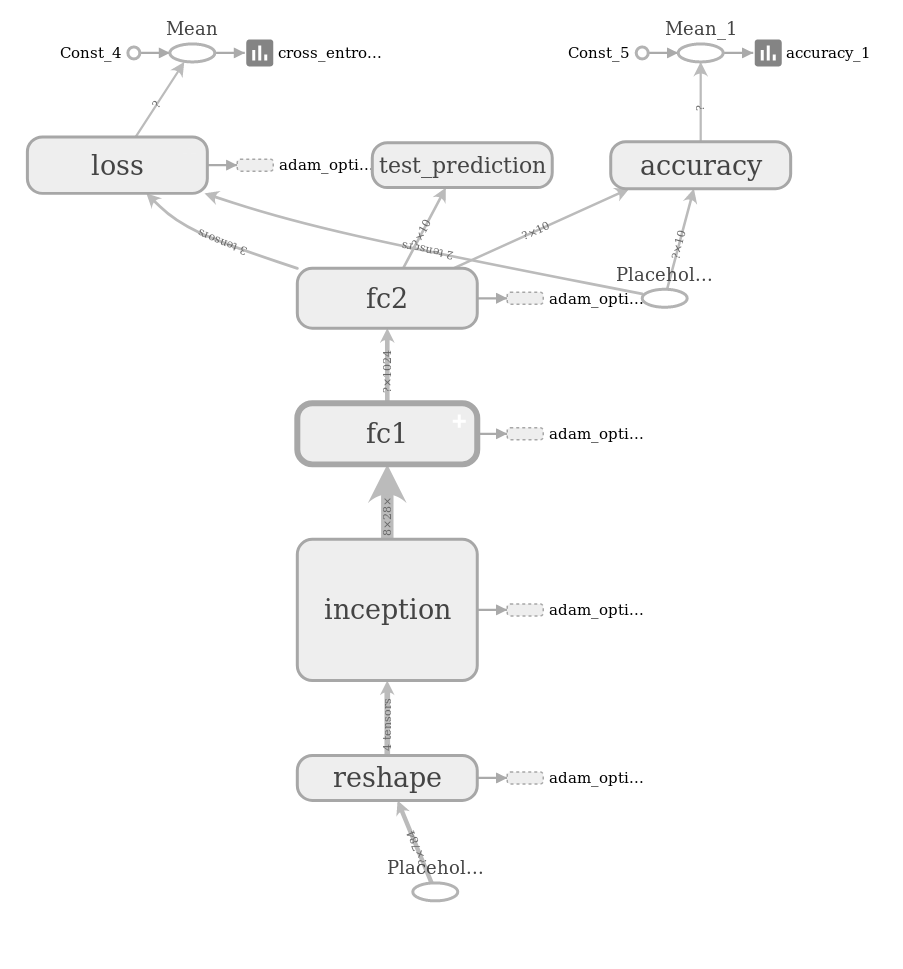
\includegraphics[width=\textwidth]{images/main_graph_inception.png}
	\label{fig:main_graph_inception}
\end{figure}
\Cref{fig:main_graph_inception} zeigt nun den Aufbau eines Netzes in dem das convolutional Layer und pooling Layer durch ein inception Layer ersetzt wurde. Dieses bekommt den gleichen Input wie das Convolution Layer im vorher beschriebenen Netz. Der Output des Inception Layers sind 4*32 features. Jedes der 4 Module des Inception Layers erzeugt 32 features der Größe 28x28, welche dann konkateniert werden. Diese Features werden dann wie vorher durch zwei fully-connected Layers weiter verarbeitet.

\section{Results}\label{sec:result}
Wir haben das Datenset, welches aus 1000 Bildern entstand aufgeteilt in ein Trainingsdatenset mit 750 Bildern und ein Testdatenset mit den übrigen 250 Bildern. Für das Training haben wir eine Batches einer Größe von 50 genutzt und für 1000 Generationen trainiert. \\

\begin{figure}
	\caption{Trainings Genauigkeit und Cross Entropy vom normalen CNN}
	\subfigure[Genauigkeit]{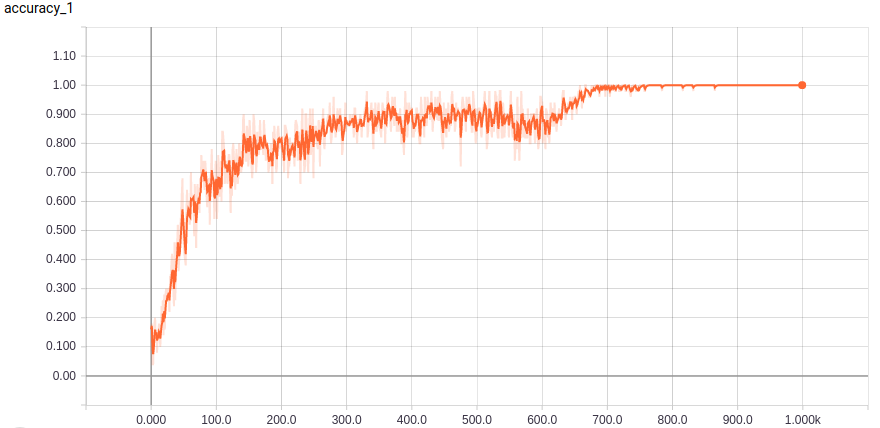
\includegraphics[width=0.49\textwidth]{images/1000_step_accuracy_conv.png}}
	\subfigure[Cross Entropy]{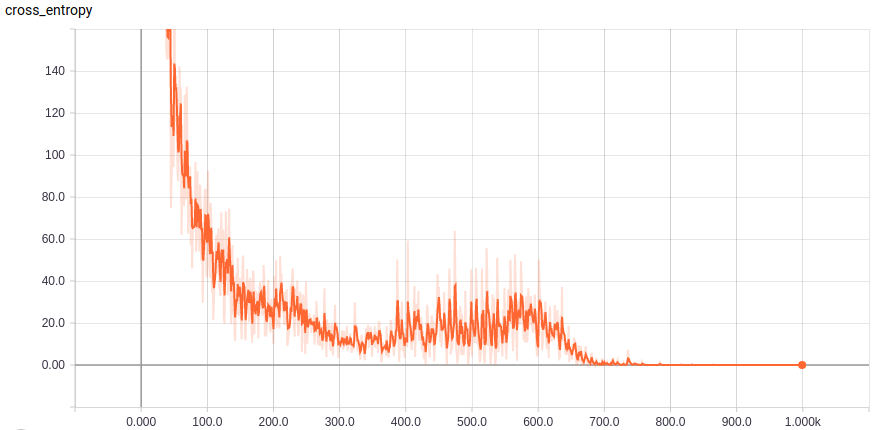
\includegraphics[width=0.49\textwidth]{images/1000_step_cross_entropy_conv.png}}
	\label{fig:conv_result_graph}
\end{figure}
In \cref{fig:conv_result_graph} sieht man die Genauigkeit und den loss, den wir mithilfe der Cross Entropy berechnet haben, von dem Neuronalen Netzwerk ohne Inception layer. Man sieht, das bereits nach ungefähr 750 Trainingsläufen die Genauigkeit relativ stabil bei 100\% liegt. Bei den Testläufen die nach diesem Training durchgeführt wurden hat das Netz ungefähr eine Genauigkeit von 85\% erreicht. Das Training von diesem Netz hat auf einem Rechner mit wenig Rechenleistung und ohne Grafikkarte nur ungefähr 5 Minuten gedauert.\\

\begin{figure}
	\caption{Trainings Genauigkeit und Cross Entropy vom CNN mit Inception layer}
	\subfigure[Genauigkeit]{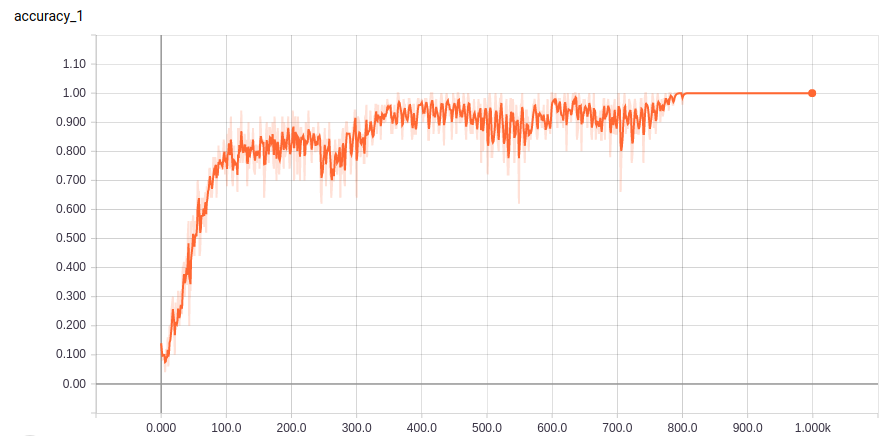
\includegraphics[width=0.49\textwidth]{images/1000_step_accuracy_inception.png}}
	\subfigure[Cross Entropy]{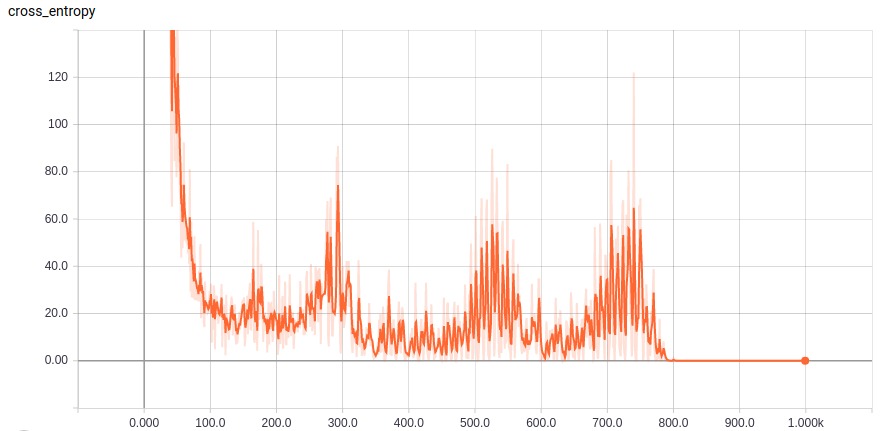
\includegraphics[width=0.49\textwidth]{images/1000_step_cross_entropy_inception.png}}
	\label{fig:inception_result_graph}
\end{figure}
\cref{fig:inception_result_graph} Zeigt die Genauigkeit und den loss von dem CNN, das ein Inception Layer anstelle der Convolution und Max Pooling Layers nutzt. Der grundsätzliche Verlauf der Graphen ist bei beiden Netzen sehr ähnlich und auch die 100 prozentige Genauigkeit wird nach einer ähnlich langen Zeit erreicht. Man sieht allerdings einige Einbrüche, insbesondere bei der Cross Entropy, in den Diagrammen des zweiten Netzes.Auch das Neuronale Netz mit dem Inception Layer erreicht nur eine Testgenauigkeit von 80\% - 85\%. Die Durchführung der 1000 Trainingsschritte hat mit diesem Netz auf dem gleichen Rechner wie bei dem ersten Netz über 30 Minuten gedauert. Also um einen Faktor von 6 länger.

\section{Discussion}\label{sec:Discussion}
Die Ergebnisse sind etwas enttäuschend, da bereits deutlich höhere Genauigkeiten für Zeichenerkennung mit anderen Convolutional Netzen erreicht wurden. Diese Verwenden häufig das MNIST Datenset \cite{mnist}, welches um ein Vielfaches größer ist als das hier genutzte Datenset. Des Weiteren ist während der Entwicklung des Netzes aufgefallen, das in dem Datenset einige Labels nicht zu dem zugehörigen Bild passen, was durch die kleine Anzahl der Daten starke Auswirkungen auf die optimal mögliche Genauigkeit hat.\\
Ein weiterer Grund für die schlechten Ergebnisse der Tests könnte sein, dass hier nur relativ kleine Netze verwendet wurden. Unsere CNN's bestanden nur aus einem Convolution- und Pooling-, beziehungsweise nur aus einem Inception Layer. Deep learning Netze haben sich in der Vergangenheit bereits als deutlich effektiver für Bildanalysen erwiesen \cite{deep_conv}. Allerdings war das für uns nicht möglich, weil uns nur sehr begrenzte Rechenleistung zur Verfügung stand. Besonders die Inception Module sind sehr rechenaufwändig, weshalb ein größeres Netz für uns nicht möglich gewesen wäre.\\

Eine Weitere Beobachtung die man von diesen Testergebnissen machen kann ist das das Netz mit dem Inception Modul keine Verbesserung der Genauigkeit bringt. Es wirkt sogar ein wenig schlechter als das andere Netz. Dazu kommt auch noch das die Laufzeit deutlich schlechter ist. Daraus kann man schließen, dass sich Inception Module nicht so gut dafür eignen um in so kleinen Netzen für Schrifterkennung eingesetzt zu werden. Ähnliche Beobachtungen kann man auch mit dem MNIST Datenset machen \cite{inception_blog}. In der Ursprünglichen Veröffentlichung wurden Inception Module in deutlich größeren Netzen und für die Analyse von komplexeren Bildern eingesetzt\cite{inception_paper}.

\section{Conclusion and Outlook}
Unsere Ergebnisse zeigen, dass Inception Layers in kleinen Netzen für die Klassifikation von Handschrift keine Vorteile gegenüber dem klassischen Aufbau von CNN's mit Convolution und Pooling Layers bringen. Außerdem konnte man erkennen, das das genutzte Datenset nicht sehr gut für das Training von Neuronalen Netzen geeignet ist, weil es zu klein ist und falsche Labels enthält.\\
Für zukünftige Arbeiten sollte man versuchen das Datenset zu erweitern und die Fehler zu korrigieren. Außerdem wäre es interessant zu untersuchen ob man bei größeren Netzen eine Verbesserung durch Inception Layers bei dieser Art der Klassifizierung beobachten kann.
\subsubsection*{Acknowledgments}
...


%%%%%%%%%%%%%%%%%%%%%%%%%%%%%%%%%%%%%%%%%%%%%%%%%%%%%%%%%%%%%%%%%%%%%%%%%%%%%%%
\bibliographystyle{splncs03}
\bibliography{paper}

All links were last followed on January 6, 2018.
%%%%%%%%%%%%%%%%%%%%%%%%%%%%%%%%%%%%%%%%%%%%%%%%%%%%%%%%%%%%%%%%%%%%%%%%%%%%%%%

\end{document}
